A single threaded test application was programmed in C++ to evaluate the FLIP water simulation with multigrid as pressure solving method. No external libraries other than the C++ standard library was used in the simulation. The graphics library OpenGL was used to display the simulation where each particle in the FLIP simulation is represented as a blue quad. The simulation generated data for display $24$ times per second.
\newline
\newline
The resolution of the grid in the test application was set to $128$ for both $N_x$ and $N_y$. The size of each side in the grid was set to $1 m$ which gives each cells a witdth of $\Delta x = 0.0078$. As can be seen in the Figure \ref{initialshapae}, the initial shape of the simulation is a halfsphere. The solid wall boundaries are placed at the grid boundaries with one grid cell as the width. No extra solids to collide against was used. Parts of the simulation can be seen in Figure \ref{simresult}. More images of the multigrid simulation can be found in Appendix A. 

\begin{figure}[ht!]
\centering

\begin{subfigure}[]{0.3\textwidth}
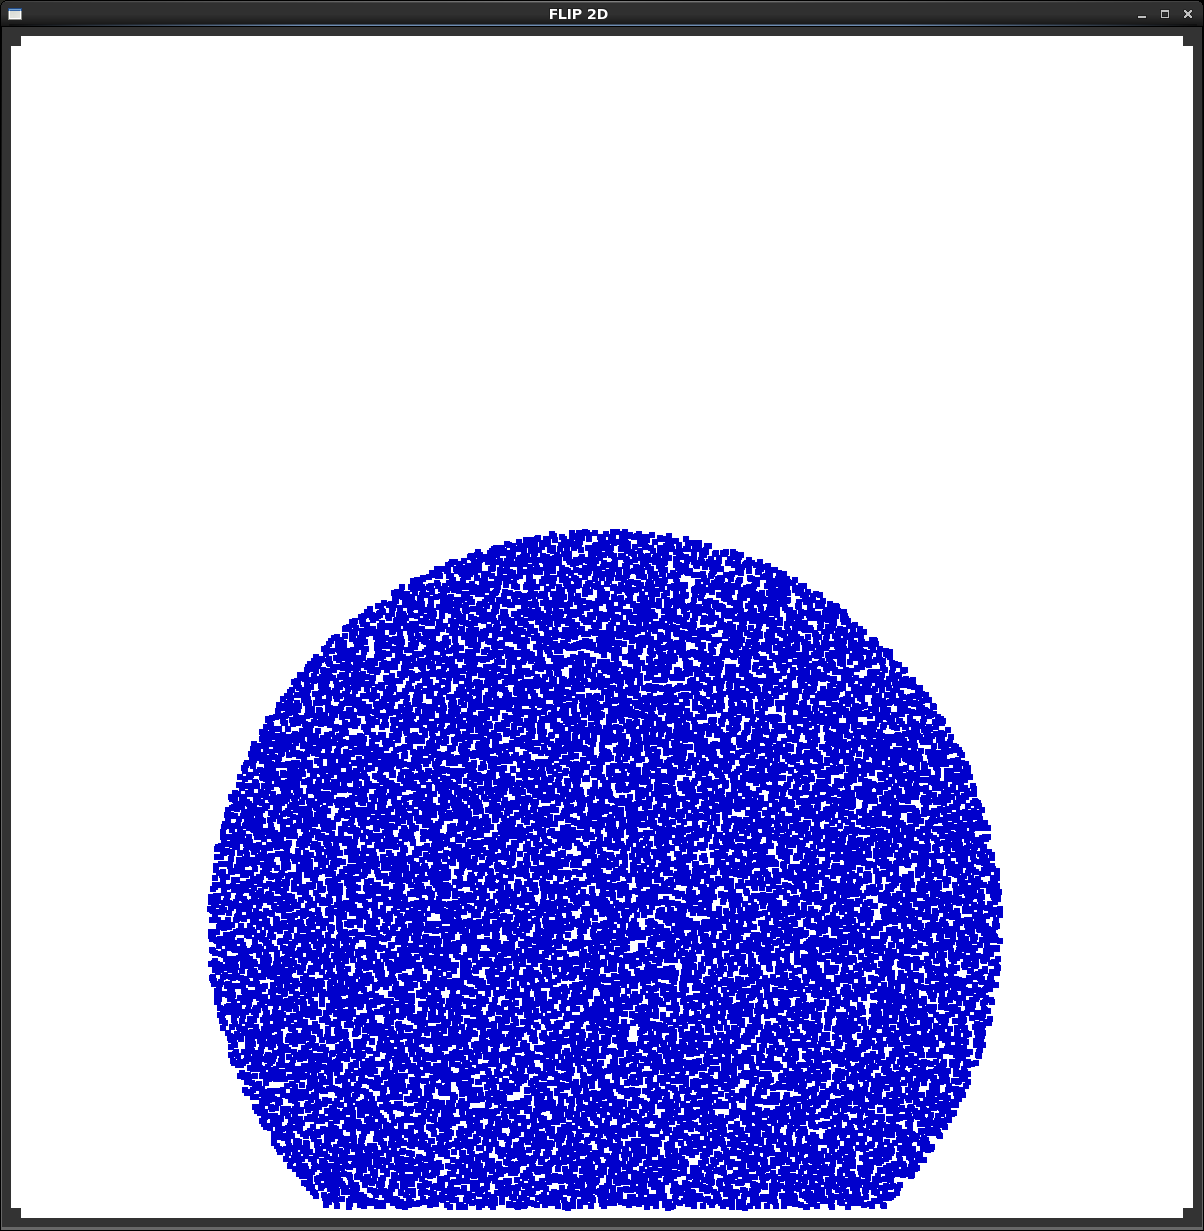
\includegraphics[height=45mm]{png/multigrid0.png}
\caption{Frame 0.}
\label{initialshapae}

\end{subfigure}
\begin{subfigure}[]{0.3\textwidth}
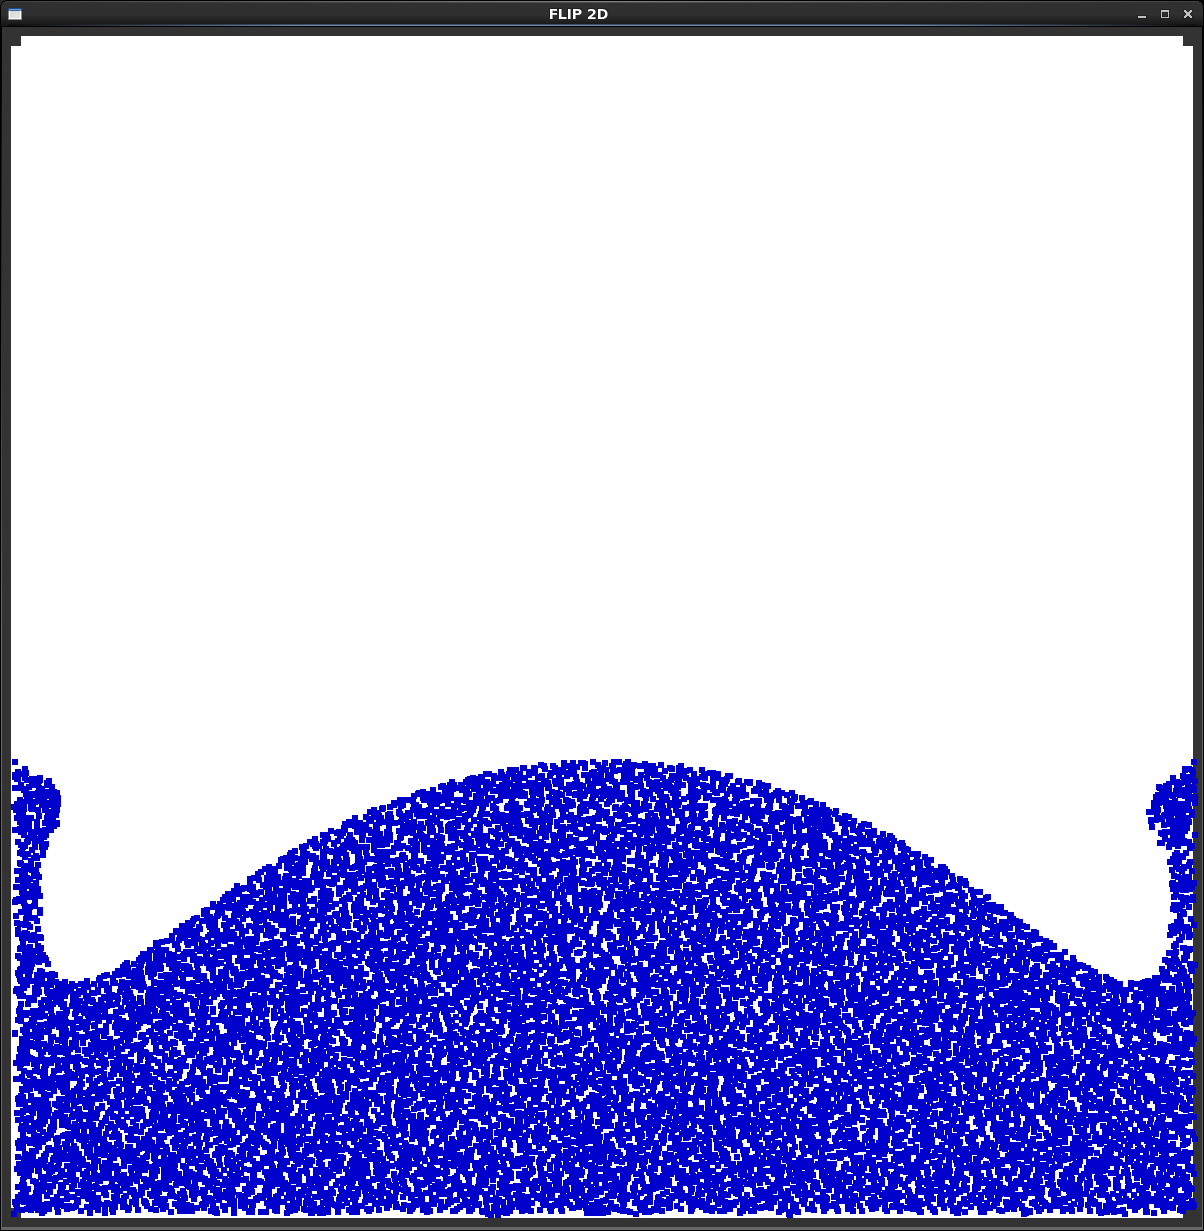
\includegraphics[height=45mm]{png/multigrid1.png}
\caption{Frame 15.}
\end{subfigure}

\begin{subfigure}[]{0.3\textwidth}
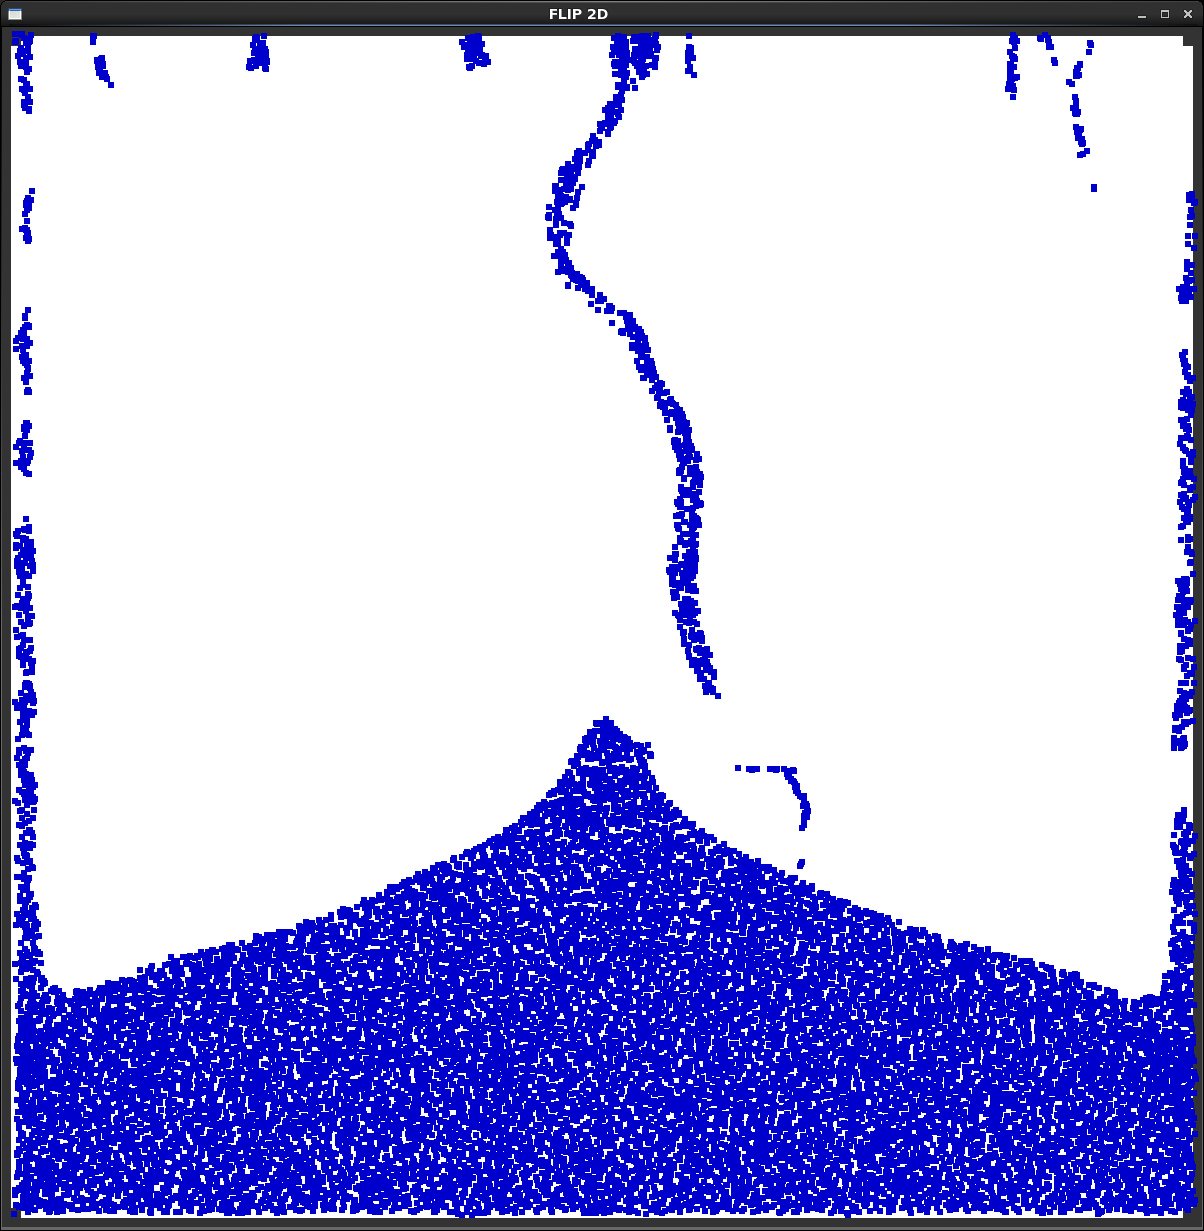
\includegraphics[height=45mm]{png/multigrid4.png}
\caption{Frame 60.}
\end{subfigure}

\caption{Results of the multigrid simulation.}
\label{simresult}
\end{figure}

The multigrid parameters used in Figure \ref{simresult} is $N_{sweep} = 10$ and $N_{\text{Full cycle}} = N_\text{V cycle} = 4$. Figure \ref{lowvshigh} shows the difference between using a low number of cycles vs a high number of cycles. When $N_{\text{Full cycle}}$ and $N_\text{V cycle}$ are set to lower values, we see volume loss artifacts.

\begin{figure}[ht!]
\centering
\begin{subfigure}[]{0.3\textwidth}
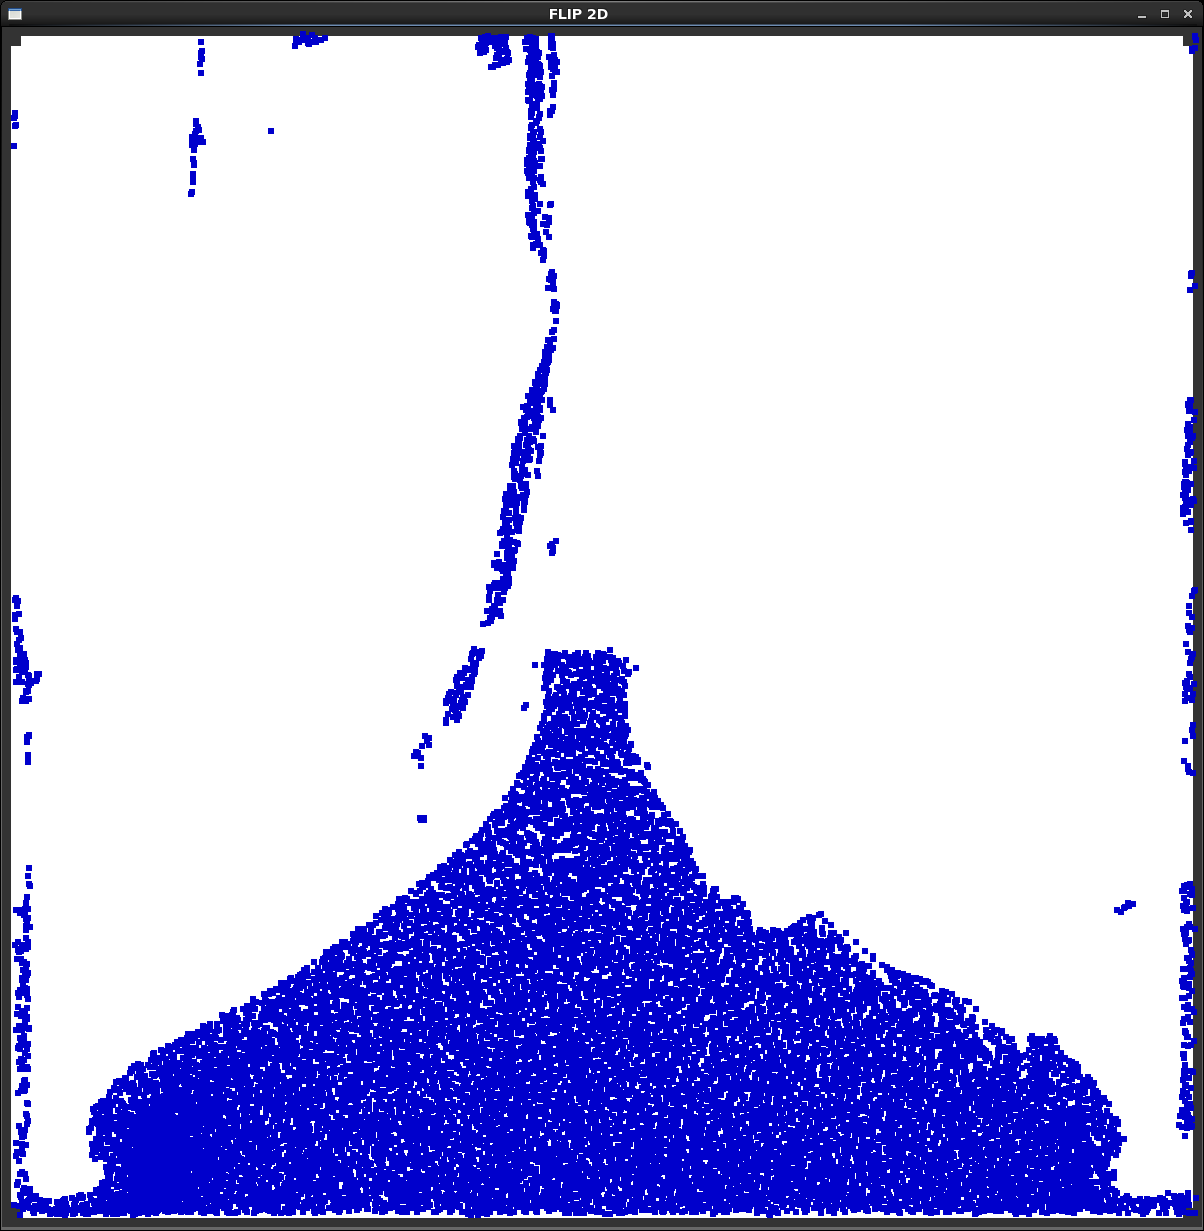
\includegraphics[height=45mm]{png/multigridN1.png}
\caption{$N_{\text{\{Full,V\} cycle}} = 1$.}
\end{subfigure}
\begin{subfigure}[]{0.3\textwidth}
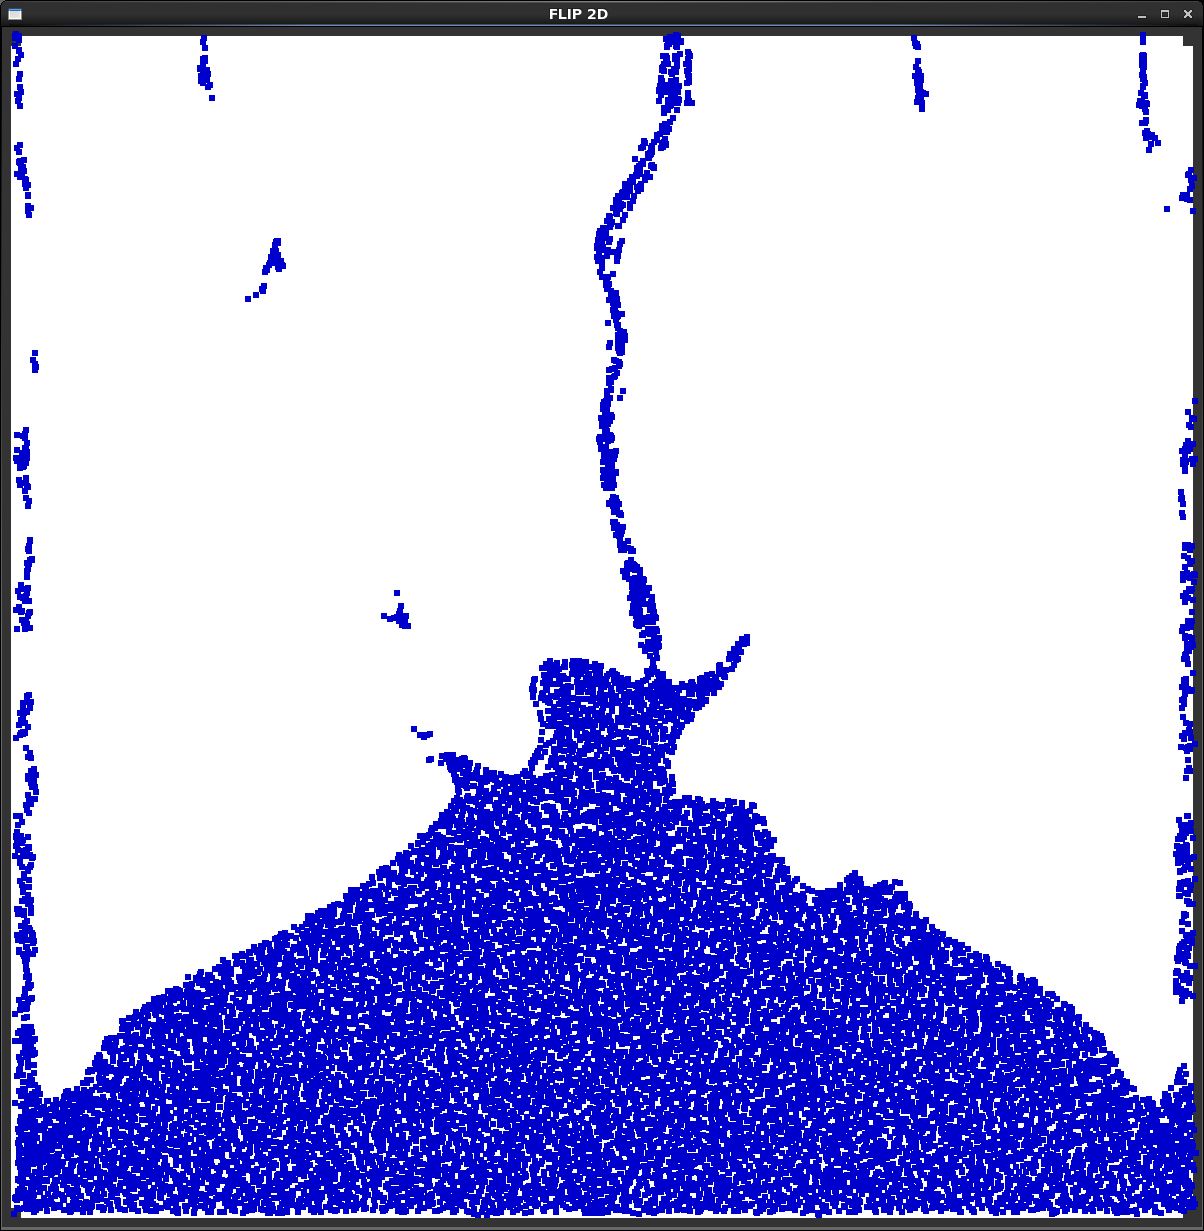
\includegraphics[height=45mm]{png/multigridN8.png}
\caption{$N_{\text{\{Full,V\} cycle}} = 8$.}
\end{subfigure}
\caption{}
\label{lowvshigh}
\end{figure}

A preconditioned conjugate gradient, PCG, pressure solver with incomplete cholesky factoziation as the preconditioner was also implemented in the test application to test correctness. For details about the implementation, one can find a detailed explenation in \cite{bridson}. A quick comparison between the multigrid method (with both cycles to be run 4 times) vs PCG can be seen in Figure \ref{pcgvsmulti}. Although different pressure solving methods, they produce solutions that look similar. Images of the full PCG simulation can be found in Appendix B. 

\begin{figure}[ht!]
\centering
\begin{subfigure}[]{0.3\textwidth}
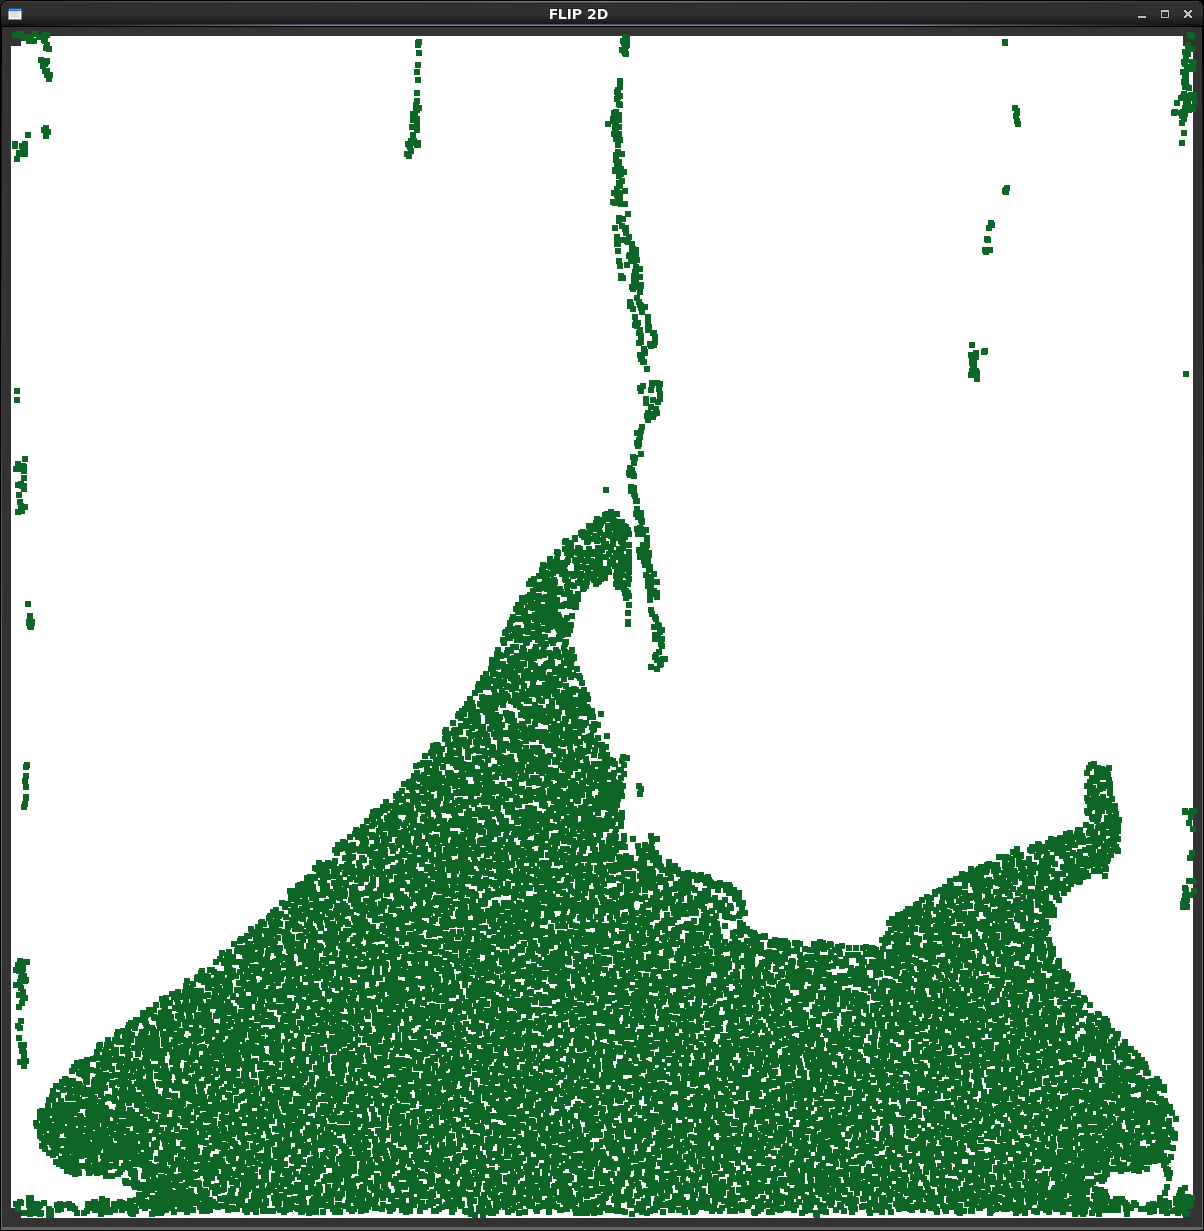
\includegraphics[height=45mm]{png/pcg5.png}
\caption{PCG.}
\end{subfigure}
\begin{subfigure}[]{0.3\textwidth}
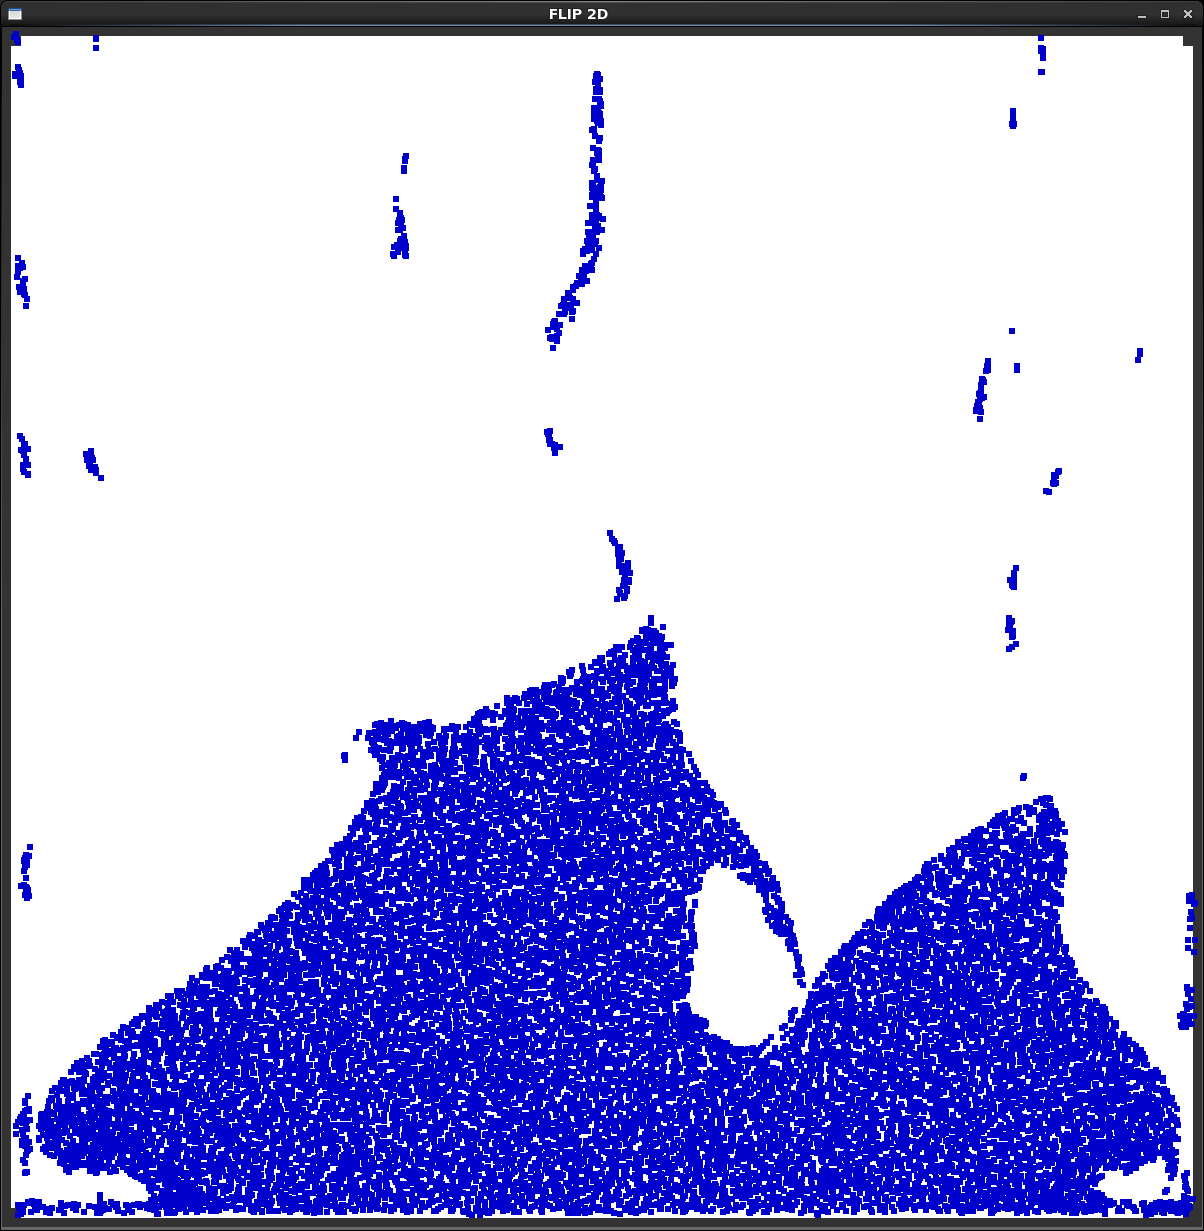
\includegraphics[height=45mm]{png/multigrid5.png}
\caption{Multigrid.}
\end{subfigure}
\caption{A comparison at frame 70 between the PCG method (green) and the multigrid method (blue).}
\label{pcgvsmulti}
\end{figure}
